%
% proposed-work.tex
%
% Copyright (C) 2022 by Universidade Federal de Santa Catarina.
%
% GNSS Networks Based on Small Satellites
%
% This work is licensed under the Creative Commons Attribution-ShareAlike 4.0
% International License. To view a copy of this license,
% visit http://creativecommons.org/licenses/by-sa/4.0/.
%

%
% \brief Proposed work chapter.
%
% \author Gabriel Mariano Marcelino <gabriel.mm8@gmail.com>
%
% \version 0.1.0
%
% \date 2021/06/14
%


\chapter{Proposed Work} \label{ch:proposed-work}

%Neste capítulo apresenta-se o trabalho proposto por essa tese. Que resumidamente consiste no estudo da viabilidade da implantação de redes de GNSS utilizando satélites de pequeno porte, podendo operar tanto em órbitas convencionais para este tipo de aplicação, mas principalmente em órbitas baixas, em altitudes que vêm sendo mais exploradas atualmente por esses tipos de dispositivos.

In this chapter, we present the work proposed by this thesis. Briefly, it consists of the study of the feasibility of implementing GNSS networks using small satellites, which can operate in both conventional orbits for this type of application, but mainly in low orbits, at altitudes that are currently being more explored by these types of devices.

\section{Orbit study}

%Além da proposta principal deste trabalho da utilização de pequenos satélites para a implantação de uma rede de GNSS, também tem-se como discussão a utilização de órbitas mais baixas para esse tipo de sistema. Atualmente as redes de GNSS já em operação trabalham em órbitas médias (MEO), na faixa dos 20000 km de altitude. Neste tipo de órbita as condições ambientais são extremamente nocivas para os subsistemas de um satélite, especialmente os componentes eletrônicos, que são submetidos a altas doses de radiação e temperaturas extremas, que provocam danos aos mesmos, diminuindo consideravelmente a sua vida útil, ou até mesmo danificando-o permanentemente.

%Para permitir a operação dos satélites neste tipo de órbita, são utilizados componentes com um certo nível de tolerância a radiação, que aguentam certas doses da mesma e permitem um maior tempo de vida. Mas esses tipos de componentes possuem um alto custo e são de difícil acesso, devido principalmente a restrições de fornecimento por parte dos países que o produzem (regulações do tipo ITAR por exemplo). Além de questões ligadas a radiação incindindo nos componentes, também há problemas ligadas a temperatura a que eles são submetidos. Em órbitas médias, temperatura negativas são comuns e requerem o uso de componentes que conseguem operar neste tipo de ambiente, como por exemplo componentes com especificações automotivas (-40 à 125 $^{\circ}$C) ou militares (-55 à 125 $^{\circ}$C). Em certos casos, também há a necessidade da utilização de controle ativo de temperatura, o que requer gasto de energia para manter integridade e/ou correto funcionamento de certos subsistemas ou componentes.

%Com a utilização de órbitas baixas (LEO), alguns desses problemas são atenuados. Devido a influência do campo magnético da Terra, os níveis de radiação em órbitas LEO são menores quando comparados com órbitas MEO. Neste caso há requisitos de tolerância menores, fazendo com que se possa utilizar componentes mais simples ou até mesmo sem classificação rad-hard. Estratégias mecânicas podem ser suficientes para a filtrar ou até mesmo barrar partículas. Além da questão de radiação, o controle térmico também torna-se mais fácil, já que a faixa de temperatura em que os satélites ficam submetidos nessa altitude é menor. Neste, dependendo do subsistema pode não haver a necessidade de um controle de temperatura ativo.

%Outro aspecto que se altera com a redução da altitude de operação, é em relação ao link de comunicação, mas especificamente o próprio sinal de GNSS gerado e transmitido pelos satélites. Como em uma órbita mais baixa, a distância entre o transmissor e um recepto em terra torna-se menor, a potência do sinal transmitido também pode ser reduzida. Desta forma, transmissores mais simples podem ser utilizados, e o consumo de energia também torna-se menor, fazendo com que no geral o satélite também possa ser reduzido fisicamente.

%E por fim, outro aspecto que se altera reduzindo a órbita de operação, é em relação ao número de satélites necessários para se ter uma cobertura total de uma certa região ou até mesmo a nível global. Neste caso, a utilização de uma órbita mais baixa trás uma desvantagem, já que são necessários mais satélites em relação a mesma situação em uma órbita do tipo MEO. Além de uma menor área de visada quando se trabalha com satélites mais baixos, o tempo de visada também torna-se menor. Neste cenário, o número de satélites necessários torna-se consideravelmente maior. Um exemplo dessa situação pode ser visto na \autoref{fig:footprint-comparison}, onde tem-se a área de visada de um satélite da rede GPS à uma altitude de aproximadamente 20000 km à esquerda, e de a área de visada de um CubeSat em órbita uma órbita de aproximadamente 600 km à direita. 

In addition to the main proposal of this work on the use of small satellites for the implementation of a GNSS network, the use of lower orbits for this type of system is also discussed. Currently, operational GNSS networks operate in medium orbits (MEO), at around 20,000 km altitude. In this type of orbit, environmental conditions are extremely harmful to satellite subsystems, especially electronic components, which are subjected to high doses of radiation and extreme temperatures that cause damage, significantly reducing their lifespan, or even permanently damaging them.

To allow satellite operation in this type of orbit, radiation-tolerant components are used, which can withstand certain doses of radiation and allow for longer lifespan. However, these types of components are expensive and difficult to obtain, mainly due to supply restrictions from countries that produce them (such as ITAR regulations). In addition to radiation-related issues affecting components, there are also temperature-related issues. In medium orbits, negative temperatures are common and require the use of components that can operate in such an environment, such as components with automotive (-40 to 125 $^{\circ}$C) or military (-55 to 125 $^{\circ}$C) specifications. In some cases, active temperature control is also required, which requires energy expenditure to maintain the integrity and/or proper functioning of certain subsystems or components.

With the use of low Earth orbits (LEO), some of these problems are mitigated. Due to the influence of the Earth's magnetic field, radiation levels in LEO are lower compared to MEO orbits. In this case, there are lower tolerance requirements, making it possible to use simpler or even non-rad-hard classified components. Mechanical strategies can be sufficient to filter or even block particles. In addition to radiation issues, thermal control also becomes easier, as the temperature range in which satellites are subjected at this altitude is smaller. In this case, depending on the subsystem, there may be no need for active temperature control.

Another aspect that changes with the reduction in operating altitude is related to the communication link, specifically the GNSS signal generated and transmitted by the satellites themselves. As the distance between the transmitter and a ground receiver becomes shorter in a lower orbit, the power of the transmitted signal can also be reduced. Thus, simpler transmitters can be used, and energy consumption also becomes lower, allowing the satellite to be physically reduced overall.

Finally, another aspect that changes by reducing the operating orbit is related to the number of satellites required to achieve full coverage of a certain region or even globally. In this case, the use of a lower orbit brings a disadvantage, as more satellites are required compared to the same situation in a MEO orbit. In addition to a smaller line-of-sight area when working with lower satellites, the line-of-sight time also becomes shorter. In this scenario, the number of required satellites becomes considerably higher. An example of this situation can be seen in \autoref{fig:footprint-comparison}, where the line-of-sight area of a GPS network satellite at an altitude of approximately 20,000 km is shown on the left, and the line-of-sight area of a CubeSat in orbit at an altitude of approximately 600 km is shown on the right.

\begin{figure}[!htb]
    \begin{center}
        \subfigure[Footprint of a GPS satellite, GPS BIIR-5 (PRN 28).\label{fig:footprint-gps}]
        {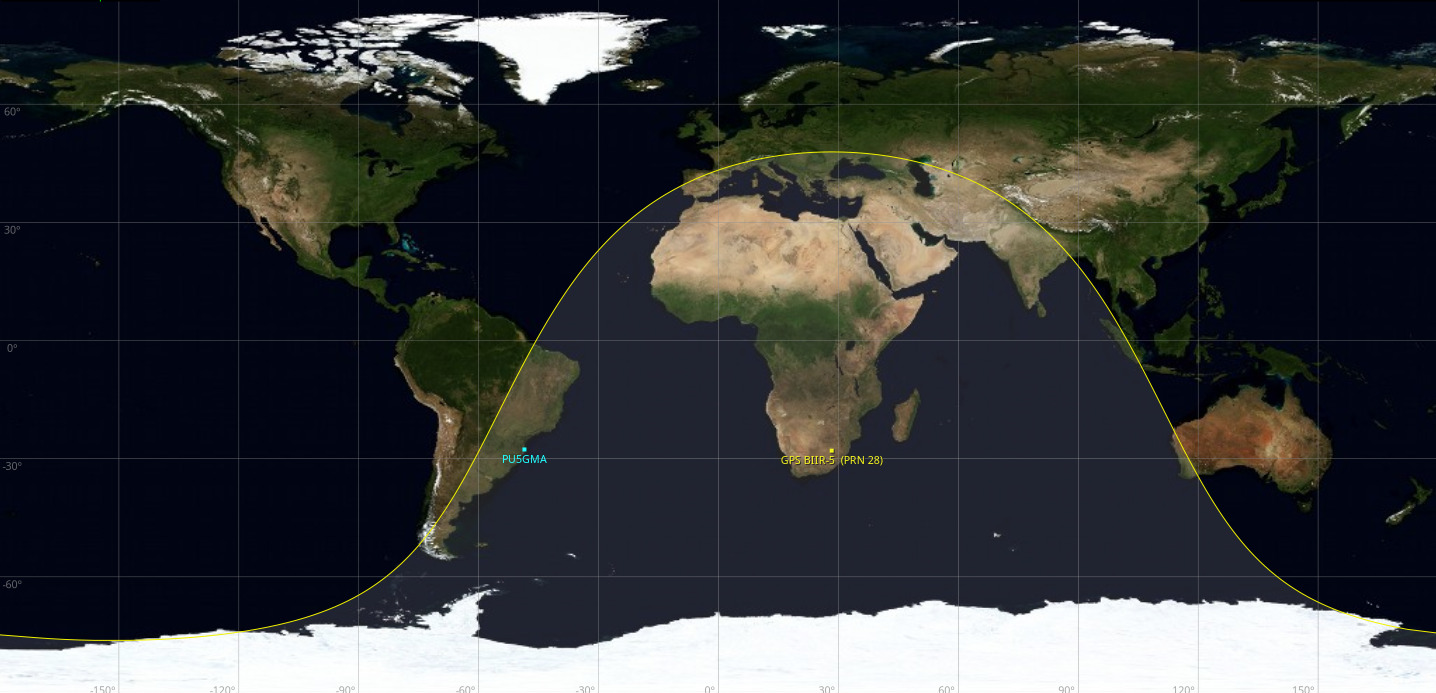
\includegraphics[width=\textwidth]{figures/footprint-gps.jpg}}
        ~
        \subfigure[Footprint of a LEO CubeSat, ITASat-1.\label{fig:footprint-itasat}]
        {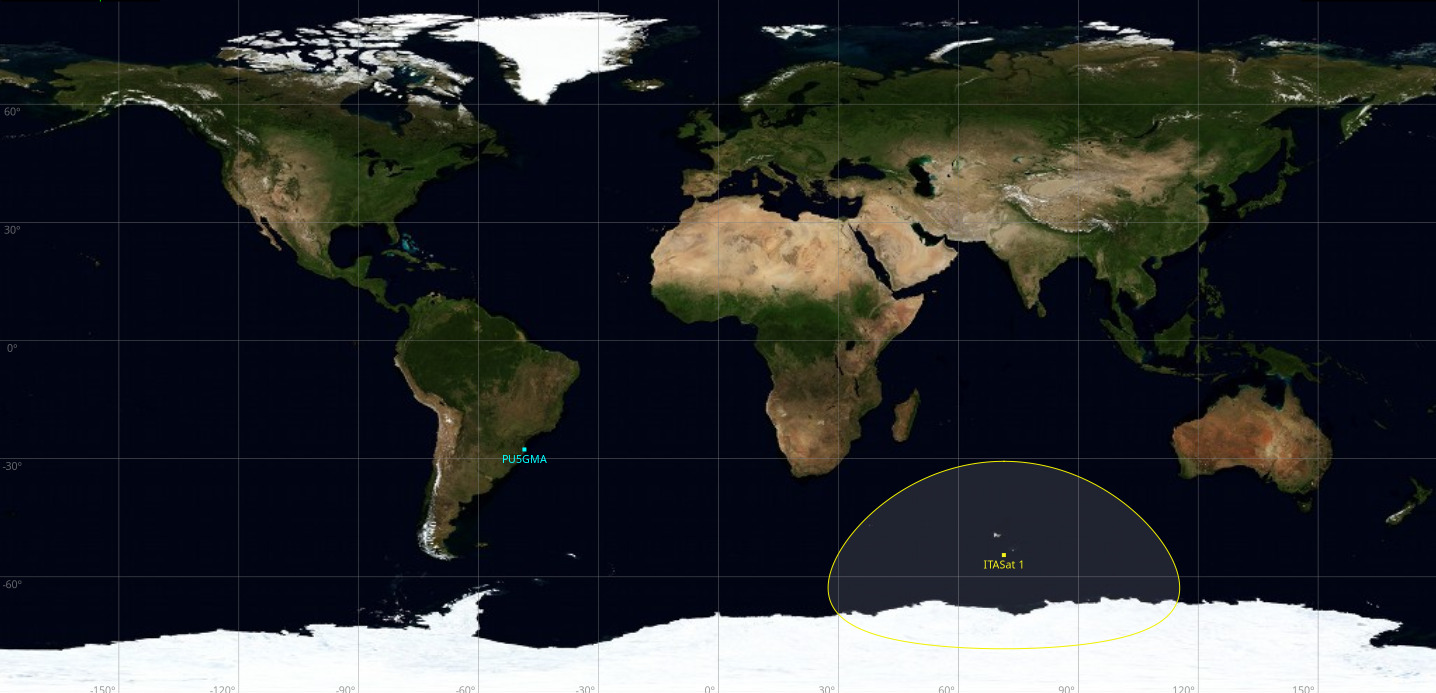
\includegraphics[width=\textwidth]{figures/footprint-itasat.jpg}}
        \caption{Comparison of the footprint area of a satellite in MEO orbit and one in a LEO orbit.}
        \label{fig:footprint-comparison}
    \end{center}
\end{figure}

\subsection{Preliminary simulations}

%Como primeiras análises de órbita, tendo como objetivo determinar principalmente o tempo de decaimento, o período para uma volta e a quantidade necessária de satélites, nesta seção apresenta-se as primeiras simulações de órbita realizadas. Para isso, utilizou-se o software GMAT, tendo como referência uma TLE do nanossatélite FloripaSat-1 \cite{marcelino2021} (modificada para uma altitude mais baixa), juntamente com os modelos de órbita e parâmetros utilizados em \cite{marino2016}. Os parâmetros de órbita adotados podem ser vistos na \autoref{tab:orbit-parameters}.

As initial orbit analyses, aiming to determine primarily the decay time, the period for one revolution, and the required quantity of satellites, this section presents the first orbit simulations conducted. For this purpose, the GMAT software was used, taking as reference a TLE of the FloripaSat-1 nanosatellite \cite{marcelino2021} (modified for a lower altitude), along with the orbit models and parameters used in \cite{marino2016}. The adopted orbit parameters can be seen in \autoref{tab:orbit-parameters}.

%To define the orbit parameters and simulate the behaviour of the satellite during its operation, the GMAT software was used \cite{gmat}. The orbit parameters was based on the FloripaSat-I TLE, but with a lower altitude. These parameters can be seen in \autoref{tab:orbit-parameters}.

\begin{table}[!ht]
    \centering
    \begin{tabular}{lcc}
        \toprule[1.5pt]
        \textbf{Parameters} & \textbf{Value} & \textbf{Unit} \\
        \midrule
        Altitude                & 550           & km \\
        Eccentricity            & 0,0015051     & $^{\circ}$ \\
        Inclination             & 97,9750       & $^{\circ}$ \\
        RAAN                    & 85,5100       & $^{\circ}$ \\
        Arg. of Perigee (AOP)   & 194,87        & $^{\circ}$ \\
        TA                      & 99,8877       & $^{\circ}$ \\
        \bottomrule[1.5pt]
    \end{tabular}
    \caption{Initial orbit parameters (adapted from FloripaSat-1).}
    \label{tab:orbit-parameters}
\end{table}

The parameters of the orbit model used in the GMAT simulation (based on the work of \cite{marino2016}) can be seen listed below:

\begin{itemize}
    \item Force model for gravitational field: ``\textit{Earth Gravitational Model 1996 (EGM96)}'' \cite{lemoine1998}
    \item Propagator: ``\textit{PrinceDorman78}''
    \item Drag coefficient: 2,2
    \item Drag atmosphere model: ``\textit{Mass Spectrometry and Incoherent Scatter (MSISE90)}'' \cite{hedin1991}
    \item Epoch: 01 Jan 2022 11:59:28.000
\end{itemize}

%Executando-se essa simulação por um período de algumas horas, chegou-se aos resultados da Figuras \ref{fig:fsat2-gmat} e \ref{fig:fsat2-gmat-groundtrack}.

Running this simulation for a few hours, the results shown in Figures \ref{fig:fsat2-gmat} and \ref{fig:fsat2-gmat-groundtrack} were obtained. The \autoref{fig:fsat2-gmat} shows the 3D representation of the obtained orbit simulation, \autoref{fig:fsat2-gmat-groundtrack} shows the ground track of the first day of operation. As can be seen, and as expected, a polar orbit with global coverage was achieved.

\begin{figure}[!ht]
    \begin{center}
        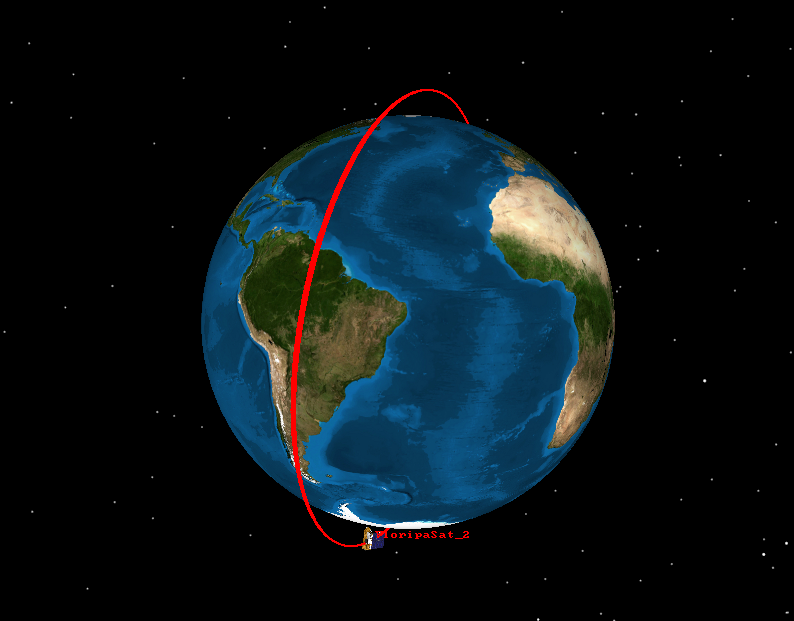
\includegraphics[width=0.6\columnwidth]{figures/fsat2-gmat.png}
        \caption{3D representation of the obtained orbit in the GMAT's simulation.}
        \label{fig:fsat2-gmat}
    \end{center}
\end{figure}

\begin{figure}[!ht]
    \begin{center}
        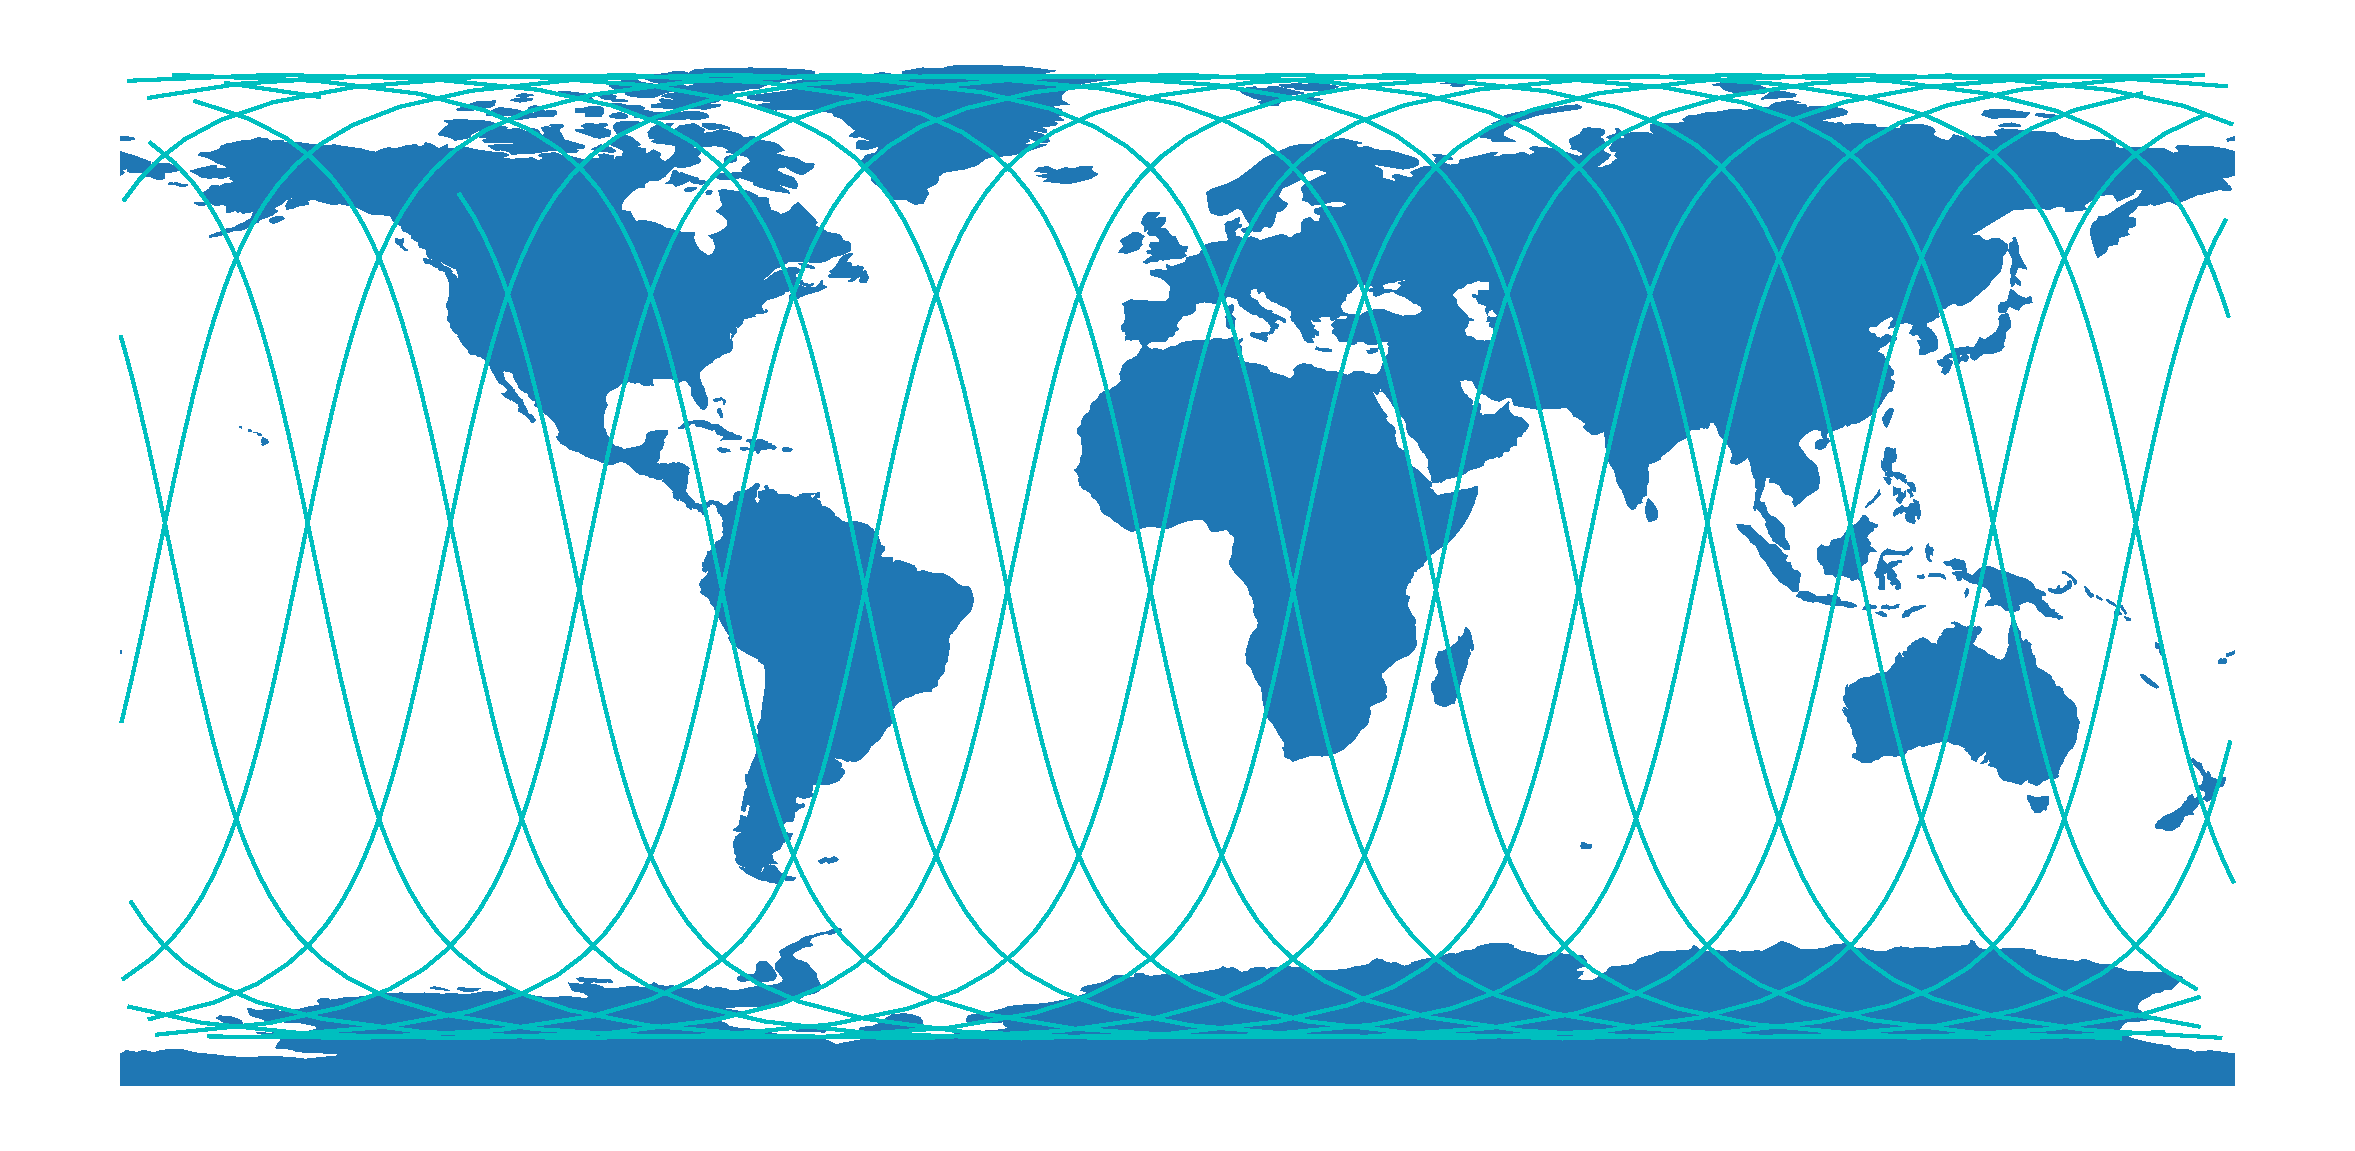
\includegraphics[width=\columnwidth]{figures/fsat2-gmat-groundtrack.pdf}
        \caption{Groundtrack of the obtained simulation.}
        \label{fig:fsat2-gmat-groundtrack}
    \end{center}
\end{figure}

The next section present some analysis based on the results obtained on the simulations executed on GMAT.

%The source files of the GMAT simulation are available in \cite{fsat2-mechanical}.

\subsection{Lifetime analysis}

Considering the same parameters presented above, with an initial altitude of 550 km, the simulations on GMAT showed that the satellite decays approximately in 2000 days ($\cong$ 5 years), as can be seen in \autoref{fig:lifetime-analysis}.

\begin{figure}[!ht]
    \begin{center}
        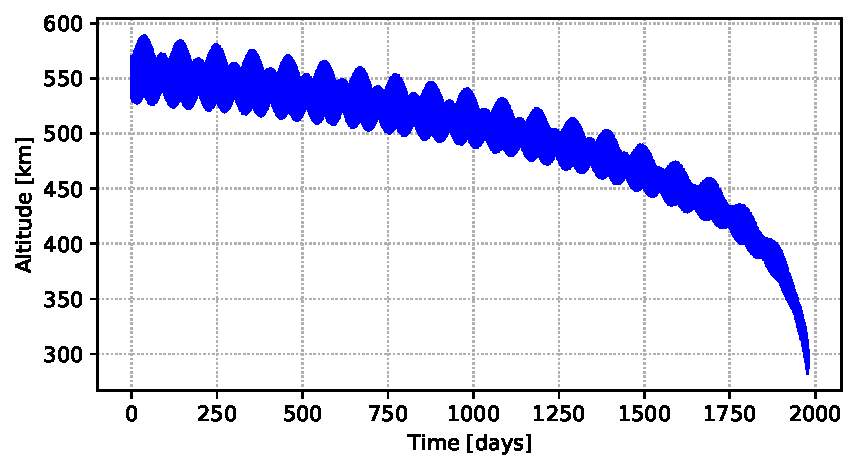
\includegraphics[width=\columnwidth]{curves/lifetime.pdf}
        \caption{Lifetime analysis on GMAT.}
        \label{fig:lifetime-analysis}
    \end{center}
\end{figure}

Lançamentos em órbitas polares e em altitude entre 500 e 600 km sãos os que tem maior disponibilidade atualmente. Sendo portanto, geralmente, os de menor custo e mais frequentes. Como oferece uma cobertura global (ou seja, é possível se comunicar com o satélite em qualquer região do globo), e um bom tempo de decaimento, torna-se ideal para missões de pequenos satélites e de baixo custo.

%Este resultado é apenas preliminar e serve apenas como uma referência. Resultados mais precisos relacionados a órbita e principalmente ao decaimento dependem de mais definições da missão, como por exemplo a data lançamento e o tamanho do satélite.

This result is only preliminary and serves as a reference only. More accurate results related to the orbit and, especially, decay depend on further mission specifications, such as the launch date and the satellite's size.

\section{Communication study}

%Um outro tipo de análise de extrema importância para o planejamento de missões satelitais, e de ainda maior importância tratando-se de um sistema de posicionamento por satélites, é a análise de comunicação. Esta análise tem como objetivo determinar a viabilidade do canal de comunicação entre o satélites e uma estação na Terra.

%Utilizando-se o método e as equações apresentadas em \autoref{sec:telecom-analysis-method}, chega-se aos resultados abaixo.

Another type of analysis of extreme importance for satellite mission planning, and of even greater importance for a satellite positioning system, is the communication analysis. This analysis aims to determine the feasibility of the communication channel between the satellites and a ground station.

By using the method and equations presented in Section \ref{sec:telecom-analysis-method}, the following results are obtained.

Fist, the distance to satellite at horizon can be obtained using \autoref{eq:horizon-distance}. Same way as used in the orbit simulation, considering an altitude of 550 km, the maximum distance between the satellite and an station on Earth, is approximately 2700 km, as can be seen in \autoref{eq:horizon-distance-result}.

\begin{equation} \label{eq:horizon-distance-result}
d = \sqrt{2\cdot 6378\cdot 550 + 550^{2}} = \mathbf{2705\ km}
\end{equation}

Considering a frequency of 900 MHz (one possible frequency band that can be used for the proposed service), the minimum and maximum FSBL is as presented in Equations \ref{eq:fslp-min-result} and \ref{eq:fspl-max-result}.

\begin{equation} \label{eq:fslp-min-result}
    FSPL^{dB}_{min} = 32,45 + 20\log\left(\frac{550}{1\ km}\right) + 20\log\left(\frac{900}{1\ MHz}\right) \cong \mathbf{146.3\ dB}
\end{equation}

\begin{equation} \label{eq:fspl-max-result}
    FSPL^{dB}_{max} = 32,45 + 20\log\left(\frac{2705}{1\ km}\right) + 20\log\left(\frac{900}{1\ MHz}\right) \cong \mathbf{160.2\ dB}
\end{equation}

This way, the FSPL can be will in the following range during a satellite pass:

\begin{equation}
    \mathbf{146.3 \leq FSPL^{dB} \leq 160.2\ dB}
\end{equation}

Considering the worst scenario with the maximum possible distance between the satellite and a receiver on Earth, a transmitter in the satellite with a output power of 30 dBm (1 W), antennas with 3 dBi of gain, and 5 dB as general losses, the power at the receiver for the link is calculated below.

\begin{equation}
    P_{r} = 30 + 3 + 3 - 160.2 - 5 = -129.2\ dBm
\end{equation}

\begin{equation}
    \mathbf{P_{r} \geq -129.2\ dBm}
\end{equation}

For calculating the SNR of the received signal, Equations \ref{eq:snr-db-with-losses} and \ref{eq:system-noise-temperature} can be used, with:

\begin{itemize}
    \item $P_{t} = 30\ dBm$
    \item $G_{t} = 3\ dBi$
    \item $G_{r} = 3\ dBi$
    \item $L_{p} = 160.2\ dB$
    \item $L_{s} = 5\ dB$
    \item $R = 1200\ bps$
    \item $T_{0} = 290\ K$
    \item $T_{r} = 290\ K$
    \item $T_{ant} = 300\ K$
    \item $F = 2\ dB$
    \item $L_{r} = 0,89\ (0,5\ dB)$
\end{itemize}

The results are presented below:

\begin{equation}
    T_{s} = 300 + \left( \frac{290 (1 - 0,89)}{0,89} \right) + \left( \frac{290 (2 - 1)}{0,89} \right) = 661,7\ K
\end{equation}

\begin{equation}
    SNR^{dB} = 30 - 30 + 3 + 3 - 160.2 - 5 + 228.6 - 28.21 - 30.79 = 10.4\ dB
\end{equation}

\begin{equation}
\mathbf{SNR^{dB} \geq 10.4\ dB}
\end{equation}

Considering the link margin as the SNR of the link minus the SNR threshold for a given bit error, the link margin of the radio links of the satellite are:

\begin{itemize}
    \item Resultant link margin: $10.4 - 9.6 = \mathbf{0.8\ dB}$
\end{itemize}

The SNR threshold was taken from \autoref{tab:link-margins}, and is the estimated value considering the BPSK modulation and a BER\nomenclature{\textbf{BER}}{Bit Error Rate.} of $10^{5}$.

As can be seen, the resultant link margin for the considered parameters is low. However, this result considers the worst-case scenario where a zero degree of elevation between the observer and the satellite is assumed. For a more realistic scenario, a higher minimum elevation should be considered. In practice, it is challenging to achieve a clear line of sight without obstacles when the satellite is at the horizon. With a higher elevation, the Free Space Path Loss (FSPL) of the link will be lower, resulting in a higher Signal-to-Noise Ratio (SNR).

Other aspects can also be considered. For example, active antennas with higher gains can be used for the system, especially on the receiver side.

\section{Required power budget}

%Com a ideia aqui proposta para a implementação de um sistema de de GNSS baseado em pequenos satélites, um das principais dificuldades de tal implementação está relacionada a geração de energia de cada satélite da rede. Como satélites de pequeno porte possuem limitações em relação a área dos painéis solares e ao armazenamento de energia, devido ao tamanho reduzido, a energia disponível para o subsistemas do satélite é limitada.

%Sendo assim, nessa seção se analisará os requisitos de energia necessários para tal sistema considerando a utilização de subsistemas comumentemente utilizados em CubeSats e encontrados a venda no mercado, e estimativas de consumo para alguns subsistemas.

%Na \autoref{tab:power-budget-subsystems}, encontram-se os subsistemas considerados para essa análise.

With the idea proposed here for the implementation of a GNSS system based on small satellites, one of the main difficulties of such implementation is related to the power generation for each satellite in the network. Since small satellites have limitations regarding the area of solar panels and energy storage, due to their reduced size, the available energy for the satellite subsystems is limited.

Therefore, in this section, we will analyze the power requirements necessary for such a system, considering the use of subsystems commonly used in CubeSats and available in the market, as well as estimates of power consumption for some subsystems.

In \autoref{tab:power-budget-subsystems}, the subsystems considered for this analysis can be found, with the respective power consumption range.

\begin{table}[!ht]
    \centering
    \begin{tabular}{lcccc}
        \toprule[1.5pt]
        \textbf{Subsystem} & \textbf{Manufacturer} & \textbf{Model} & \textbf{Consumption [mW]} \\
        \midrule
        OBDH     & GomSpace & NanoMind A3200 & 170 \\
        EPS      & GomSpace & NanoPower P60  & 160 \\
        Battery  & GomSpace & NanoPower BP4  & 50-7000 \\
        TMTC     & GomSpace & NanoCom AX100  & 300-3300 \\
        Antenna  & ISISpace & AntS           & 35-1800 \\
        ADCS     & ISISpace & iMTQ           & 175-1200 \\
        GNSS Transmitter & \multicolumn{2}{c}{Custom model} & 4720 \\
        \bottomrule[1.5pt]
    \end{tabular}
    \caption{Power consumptions reference.}
    \label{tab:power-budget-subsystems}
\end{table}

%Para o transmissor de GNSS, conforme apresentado na \autoref{sec:ionospheric-delay}, se considerará dois transmissores operando em tempo integral. Como base para os cálculos, será considerado o consumo de um transmissor operando em Banda-S disponível no mercado e voltado especificamente para CubeSats (modelo NanoCom AX2150, da GomSpace \cite{ax2150}). Este apresenta um consumo de 2200 mW durante a transmissão, e de 500 mW durante o modo de recepção. Já para a parte da referência de tempo, se utilizará como base os valores de consumo do oscilador de rubídio CSAC SA.45S da Microchip. Conforme descrito na documentação do mesmo, este apresenta um consumo de 120 mW durante uma operação normal. Para as antenas dos transmissores, também se considerará o consumo de uma antena para Banda-S disponível comercialmente para CubeSats (modelo NanoCom AM2150-P, da GomSpace \cite{am2150-p}). Neste caso, por tratar-se de uma antena passiva, o consumo considerado será zero. Por fim, para outros possíveis elementos de payload como microcontrolador e sensores, se considerará um consumo de 200 mW. Os valores de consumo considerados para o payload de GNSS estão descritos na \autoref{tab:power-gnss-payload}.

For the GNSS transmitter, as presented in \autoref{sec:ionospheric-delay}, two transmitters operating full-time will be considered. As a basis for the calculations, the power consumption of a commercially available Band-S transmitter specifically designed for CubeSats will be taken into account (NanoCom AX2150 model, from GomSpace \cite{ax2150}). This transmitter has a consumption of 2200 mW during transmission and 500 mW during reception mode. As for the time reference component, the power consumption values of the CSAC SA.45S rubidium oscillator from Microchip will be used as a basis. According to the documentation, this oscillator has a consumption of 120 mW during normal operation. For the transmitter antennas, the power consumption of a commercially available S-Band antenna for CubeSats will also be considered (NanoCom AM2150-P model, from GomSpace \cite{am2150-p}). In this case, as it is a passive antenna, the consumption will be considered as zero. Finally, for other potential payload elements such as microcontrollers and sensors, a consumption of 200 mW will be considered. The power consumption values considered for the GNSS payload are synthetized in \autoref{tab:power-gnss-payload}.

\begin{table}[!ht]
    \centering
    \begin{tabular}{lcccc}
        \toprule[1.5pt]
        \textbf{Item} & \textbf{Quantity} & \textbf{Consumption [mW]} \\
        \midrule
        RF transmitter  & 2 & 2200 \\
        Clock reference & 1 & 120 \\
        Antenna         & 2 & 0 \\
        Others          & 1 & 200 \\
        \cmidrule{2-3}
        Total           & \multicolumn{2}{c}{4720} \\
        \bottomrule[1.5pt]
    \end{tabular}
    \caption{Estimated power consumption of the GNSS payload.}
    \label{tab:power-gnss-payload}
\end{table}

%Para o duty cycle e modos de operação se utilizará como referência o utilizado em outras missões de CubeSat. Neste caso, assume-se os módulos de serviço operando da mesma forma que em um CubeSat em uma missão ``genérica''.

For the duty cycle and operating modes, the reference will be based on those used in other CubeSat missions. In this case, it is assumed that the service modules operate in the same way as in a ``generic'' CubeSat mission, with the TMTC in reception mode most of the time, the ADCS operating just with small attitude corrections and the battery heater activated only during eclipses. The \autoref{tab:power-duty-cycle} presents the power consumptions and respective duty cycles.

\begin{table}[!ht]
    \centering
    \begin{tabular}{lcc}
        \toprule[1.5pt]
        \textbf{Subsystem} & \textbf{Duty Cycle [\%]} & \textbf{Power [mW]} \\
        \midrule
        OBDH                  & 100 & 170 \\
        TMTC (RX)             & 95  & 300 \\
        TMTC (TX)             & 5   & 3300 \\
        EPS                   & 100 & 160 \\
        Battery (idle)        & 90  & 50 \\
        Battery (heater full) & 10  & 7000 \\
        ADCS (idle)           & 90  & 175 \\
        ADCS (full actuation) & 10  & 1200 \\
        Antenna (deployment)  & 0   & 1800 \\
        Antenna (deployed)    & 100 & 35 \\
        Payload GNSS          & 100 & 4720 \\
        \cmidrule{2-3}
        Satellite             & \multicolumn{2}{c}{$\cong$ 6526 mW} \\
        \bottomrule[1.5pt]
    \end{tabular}
    \caption{Power consumption and duty cycle of each subsystem, and average total power of the satellites.}
    \label{tab:power-duty-cycle}
\end{table}

As can be seen from \autoref{tab:power-duty-cycle}, an average power consumption of 6526 mW was achieved for the considered system. This value is highly influenced by the power consumption of the GNSS payload, which is not the highest in the system but has a duty cycle of 100 \%. For a global GNSS system, it is expected that the transmitters are always transmitting the timing data.

With the estimated power consumption, the required area of solar panels can be calculated, and consequently, the minimum size of the satellite can be defined.

Using the method of \cite{rigo2023}, with a solar irradiance of 1367 W/m$^{2}$, and considering the solar cell CTJ30 from Cesi \cite{ctj30} (29.5 \% of efficiency and 0.003015 m$^{2}$ of area), the average total generated power for various values of solar panel area was achieved. The results can be seen in \autoref{fig:sp-area-vs-pwr}.

\begin{figure}[!ht]
    \begin{center}
        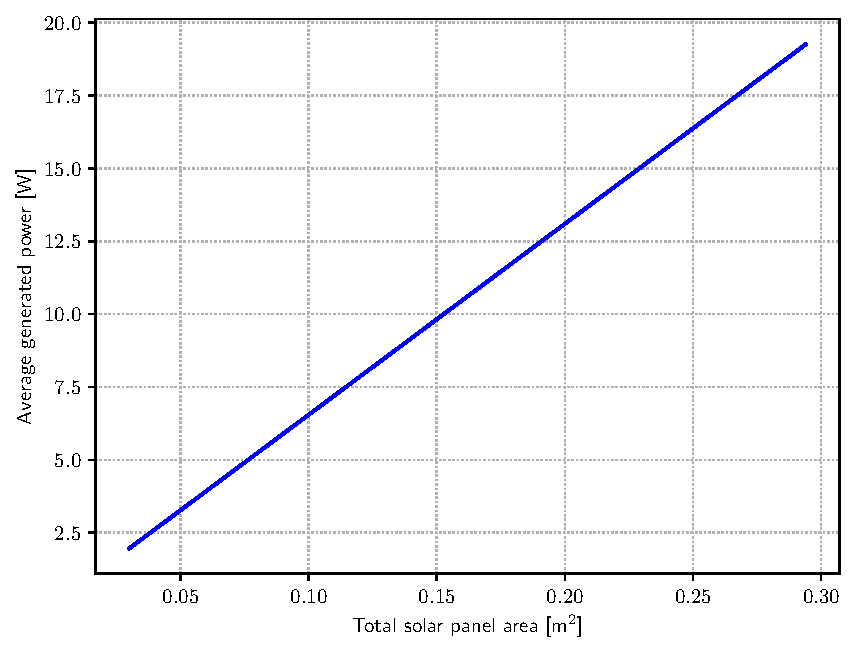
\includegraphics[width=0.8\columnwidth]{curves/sp-area-vs-pwr.pdf}
        \caption{Simulated generated power of the solar panels.}
        \label{fig:sp-area-vs-pwr}
    \end{center}
\end{figure}

Considering the power requirement presented in \autoref{tab:power-duty-cycle}, from the graph of \autoref{fig:sp-area-vs-pwr}, a total solar panel area of approximately 0.1 m$^{2}$ is required for the given system.

%Considerando um satélite sem mecanismos de abertura de painéis solares, ou seja, só com painéis fixos, instalados nas suas faces e cobrindo todas as laterais, a área mínima obtida equivale a um CubeSat entre 3 e 6U. Considerando que o padrão CubeSat não prevê a existência de satélites 4 ou 5U, chega-se ao resultado que é necessário pelo menos um CubeSat de tamanho 6U para esse sistema operando nas condições apresentadas.

%Considerando a possibilidade do uso de mecanismos de abertura de painéis, ou seja, painéis extras que são abertos após o lançamento do satélite, o uso de um CubeSat 3U também seria possível.

Considering a satellite without mechanisms for solar panel deployment, that is, only with fixed panels installed on its faces and covering all sides, the minimum area obtained corresponds to a CubeSat between 3U and 6U. Considering that the CubeSat standard does not provide for the existence of 4U or 5U satellites, the result is that at least a 6U-sized CubeSat is necessary for this system to operate under the presented conditions.

Considering the possibility of using mechanisms for panel deployment, that is, additional panels that are opened after the satellite is launched, the use of a 3U CubeSat would also be possible.

%Desta maneira, para um satélite 6U chega-se aos seguintes resultados da \autoref{tab:sp-power-6u-results} em relação a geração de energia.

In this way, for a 6U satellite, the following results from \autoref{tab:sp-power-6u-results} are obtained regarding power generation.

\begin{table}[!ht]
    \centering
    \begin{tabular}{lc}
        \toprule[1.5pt]
        \textbf{Parameter} & \textbf{Value} \\
        \midrule
        Peak power                  & 15093 mW \\
        Average power (orbit)       & 8688 mW \\
        Average power (sunlight)    & 13770 mW \\
        Orbit period                & 6018 sec \\
        Sun light period            & 3712 sec \\
        Eclipse period              & 2124 sec \\
        \bottomrule[1.5pt]
    \end{tabular}
    \caption{Results of power generation simulation for a 6U CubeSat.}
    \label{tab:sp-power-6u-results}
\end{table}

%O gráfico da \autoref{fig:sp-input-power-6u} ilustra a geração de energia por face e total durante uma órbita completa para o caso considerado.

The curves in \autoref{fig:sp-input-power-6u} illustrates the energy generation per face and total during a complete orbit for the considered case.

\begin{figure}[!ht]
    \begin{center}
        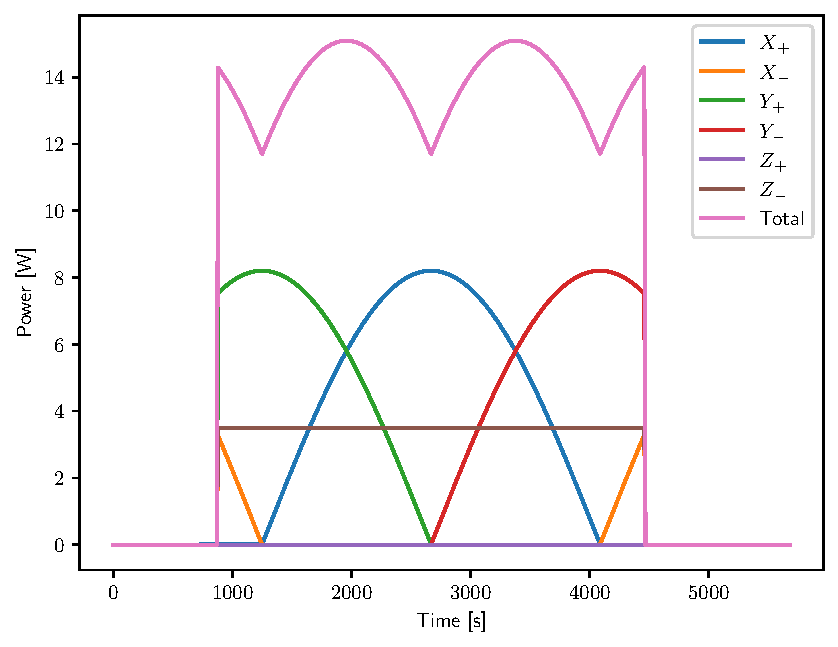
\includegraphics[width=0.8\columnwidth]{curves/sp-input-power-6u}
        \caption{Simulated input power of a 6U CubeSat.}
        \label{fig:sp-input-power-6u}
    \end{center}
\end{figure}

%Por fim, considerando a energia gerada e a consumida, chega-se a uma margem de 2162 mW, ou aproximadamente 25 \%. Esta margem é suficiente considerando-se a degradação dos painéis solares ao longo da missão, e possíveis alteração de projeto, com a remoção de células solares para a instalação de sensores ou antenas. Ou até mesmo a instalação de outros payloads ou subsistemas no mesmo satélite.

Finally, considering the generated and consumed energy, a margin of 2162 mW, or approximately 25 \%, is reached. This margin is sufficient considering the degradation of the solar panels throughout the mission, and possible design changes, such as the removal of solar cells for the installation of sensors or antennas. It also accounts for the installation of other payloads or subsystems on the same satellite.

\section{Possible solutions}

%Nesta seção apresentam-se possíveis soluções para a implementação do trabalho proposto, considerando-se os principais aspectos técnicos necessários para a implementação de um sistema desse tipo conforme as questões apresentadas até então.

In this section, possible solutions are presented for the implementation of the proposed work, considering the main technical aspects necessary for the implementation of such a system, according to the issues presented so far.

\subsection{Clock reference}

As previously mentioned, one of the main sources of error in a GNSS system is the clock reference of the signal transmitter (at the satellite side). In this section, some technologies commonly used in time reference circuits are presented, as well as a discussion of the accuracy of each system and the feasibility of using it in the system discussed here.

%\begin{enumerate}
%    \item Quartz oscilators: $\pm$1 sec a cada 30 dias
%    \item TCXO (Temperature Compensated Crystal Oscillators):
%    \item OCXO (Oven Controlled Crystal Oscillators):
%    \item RbXO (Osciladores de rubídio): $\pm$1 sec a cada 32000 anos.
%    \item Osciladores de césio:
%    \item GPSDO (GPS Disciplined Oscillator):
%\end{enumerate}

\subsubsection{Quartz oscillators (XO)}

%Os osciladores baseados diretamente em cristais como o quartzo, são os tipos de osciladores mais comuns utilizados hoje em die e estão entre os que possuem a menor precisão, perdendo somente para osciladores baseados em circuitos LC. Este tipo pode ser encontrado vastamente no mercado em diversas configurações e tamanho, além de possuir um baixo custo e consumo de energia. Mas em contrapartida é sensível a variações de temperatura, sendo não recomendado para aplicações que requerem alta precisão na frequência de saída. Devido a essas características, este tipo de oscilador não é adequado para ser utilizado como referência para um sistema de GNSS.

Oscillators based directly on crystals such as quartz are the most common types of oscillators used today and are among those with the lowest precision, second only to oscillators based on LC circuits. This type can be widely found in the market in various configurations and sizes, as well as having low cost and energy consumption. However, on the other hand, it is sensitive to temperature variations and is not recommended for applications that require high precision in the output frequency. Due to these characteristics, this type of oscillator is not suitable for use as a reference for a GNSS system.

\subsubsection{Temperature Compensated Crystal Oscillators (TCXO)}

TCXO (Temperature Compensated Crystal Oscillator) is a type of oscillator used in electronic circuits to provide a stable and accurate frequency reference. They work by using a quartz crystal as the resonating element, which vibrates at a specific frequency when electrical voltage is applied to it. This frequency can be used as a reference clock signal for timing and synchronization purposes.

However, the frequency of a quartz crystal is affected by temperature changes, leading to frequency drift and decreased accuracy. To overcome this limitation, TCXOs incorporate a temperature compensation mechanism that adjusts the frequency of the crystal based on the temperature. This can be achieved through various methods, including using a thermistor to measure the temperature and controlling the voltage applied to the crystal, or using a temperature-controlled oven to maintain the crystal at a constant temperature.

The result is a highly stable frequency source that can maintain a high level of accuracy even in harsh operating environments, making TCXOs ideal for use in various applications, such as GPS receivers, cell phones, and other portable devices that require accurate timekeeping.

Despite being significantly more accurate than a common crystal oscillator, this still is not a suitable type to be used as a reference in a GNSS system.

\subsubsection{Oven Controlled Crystall Oscillators (OCXO)}

%OCXOs são osciladores que utilizam uma câmara fechada e com a temperatura controlada para manter a estabilidade em cristais de quartzo. A ideia é manter o cristal em uma temperatura constante para evitar desvios na frequência de oscilação do mesmo por variações de temperatura.

%Devido a característica do controle ativo de temperatura, o consumo energético deste tipo de oscilador é alto em comparação com outros osciladores baseados em cristais. O consumo pode chegar a algumas unidades de watts dependendo da temperatura externa do dispositivo. Normalmente, o cristal é mantido numa temperatura de 75 $^{\circ}$C, por cristais de quartzo apresentarem melhores características de funcionamento nessa faixa. Devido a isso, para aplicações que operam em temperatura ambiente ou baixas temperaturas (como um satélite operando no espaço), o consumo de energia deste tipo de oscilador será elevado.

%Outra característica importante é o seu tamanho, devido ao controle de temperatura, normalmente o volume deste tipo de oscilador é maior dentro da classe dos modelos baseados em cristais, e normalmente não é utilizado em dispositivos portáteis ou baseados em bateria. Apesar destas características, este tipo de oscilador é o que possuí a maior precisão possível dos osciladores baseados em cristais, ficando na faixa entre $2 \times 10^{-8}$ e $5 \times 10^{-7}$ dependendo da faixa de frequência em operação \cite{mancini2004}. Um OCXO instalado em uma placa de circuito impresso pode ser visto na \autoref{fig:ex-ocxo}

OCXOs are oscillators that use a closed chamber with controlled temperature to maintain stability in quartz crystals. The idea is to keep the crystal at a constant temperature to avoid deviations in its oscillation frequency due to temperature variations.

Due to the active temperature control characteristic, the energy consumption of this type of oscillator is high compared to other crystal-based oscillators. Consumption can reach a few watts depending on the external temperature of the device. Normally, the crystal is kept at a temperature of 75 $^{\circ}$C, as quartz crystals exhibit better performance characteristics in this range. Due to this, for applications that operate at ambient or low temperatures (such as a satellite operating in space), the energy consumption of this type of oscillator will be high.

Another important characteristic is its size. Due to the temperature control, the volume of this type of oscillator is usually larger within the class of crystal-based models and is not normally used in portable or battery-based devices. Despite these characteristics, this type of oscillator has the highest possible precision among crystal-based oscillators, ranging between $2 \times 10^{-8}$ and $5 \times 10^{-7}$ depending on the operating frequency range \cite{mancini2004}. An OCXO installed on a printed circuit board can be seen in \autoref{fig:ex-ocxo}.

\begin{figure}[!ht]
    \begin{center}
        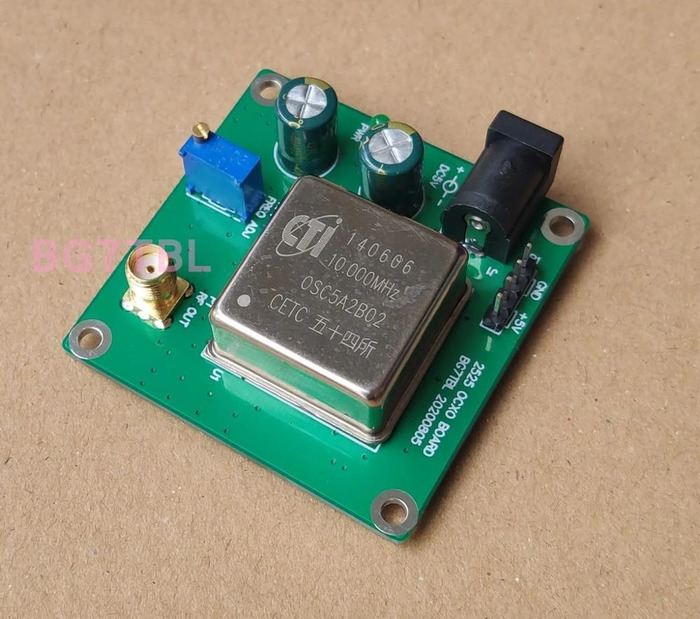
\includegraphics[width=0.5\columnwidth]{figures/ex-ocxo.jpg}
        \caption{OCXO installed on a printed circuit board.}
        \label{fig:ex-ocxo}
    \end{center}
\end{figure}

\subsubsection{Rubidium oscillators (RbXO)}


Rubidium oscillators are a type of frequency reference that use the resonant frequency of rubidium-87 atoms to generate a stable and accurate time signal. They work by confining a cloud of rubidium atoms in a small chamber and applying a magnetic field to the cloud. This magnetic field causes the rubidium atoms to transition between two energy levels, emitting or absorbing light at a very specific frequency, known as the resonant frequency of rubidium-87.

A microwave generator is used to excite the rubidium atoms, and the frequency of the generator is then locked to the resonant frequency of the rubidium atoms. The microwave generator acts as a frequency reference, and the frequency output of the generator can be used as a highly stable and accurate clock signal.

Rubidium oscillators offer a number of advantages over other types of frequency references, including high stability, low aging rate, and low sensitivity to environmental factors such as temperature and pressure changes. They are widely used in a variety of applications, including GPS systems, scientific instrumentation, and telecommunications equipment.

Rubidium oscillators are the cheapest in the class of oscillators used in atomic clocks. They are considered a secondary frequency standard, unlike Cesium oscillators which are more precise and considered primary.

Oscillators of this type are currently readily available on the market, with some examples being the Microchip SA-45S models \cite{sa45s}, which can be seen in \autoref{fig:microchip-csac}.

\begin{figure}[!ht]
    \begin{center}
        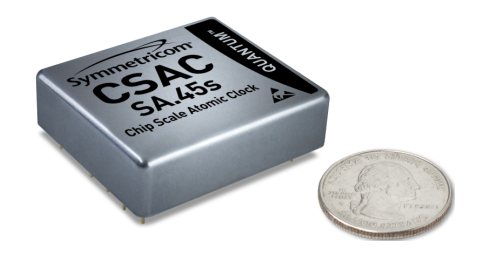
\includegraphics[width=0.7\columnwidth]{figures/microchip-csac}
        \caption{Microchip CSAC SA.45S atomic clock.}
        \label{fig:microchip-csac}
    \end{center}
\end{figure}

Considering factors such as physical size, power consumption, and cost, this type of oscillator is a good option to be considered as a reference for a small satellite-based GNSS system.

\subsubsection{Cesium oscillators}

Cesium atomic clocks are highly precise timekeeping devices that use the vibration frequency of cesium-133 atoms to measure the passage of time. They are considered the standard for time and frequency measurements, as their accuracy is several orders of magnitude better than that of traditional quartz clocks. Cesium atomic clocks are used in a variety of applications, including navigation, telecommunications, and scientific research, and they play a critical role in maintaining Coordinated Universal Time (UTC), the international time standard.

Cesium atomic clocks work by utilizing the vibrational frequency of cesium-133 atoms in a highly controlled environment. The atoms are first excited by a microwave frequency and then allowed to settle into their ground state. As the atoms transition from their excited state to their ground state, they emit electromagnetic radiation at a very specific frequency. This frequency, known as the hyperfine transition frequency of cesium-133, serves as the standard for measuring the passage of time.

In a cesium atomic clock, the atoms are confined in a container called an oven and heated to a high temperature to increase their motion and make the hyperfine transitions easier to detect. The frequency of the microwave radiation that excites the atoms is measured using a sensor called a frequency counter, and this frequency is compared to a reference frequency source to determine the exact time. The whole process is repeated several times per second to maintain a highly accurate and stable measurement of time. The resulting timekeeping system is able to maintain a precision of a few parts in $10^{14}$, making cesium atomic clocks the most accurate timekeepers currently available.



\subsubsection{GPS disciplined oscillators (GPSDO)}

%Um GPSDO, ou GPS disciplined oscillator, é a combinação de um receptor de sinais GPS (ou qualquer outra rede de GNSS) com um oscilador comum, como qualquer um dos tipos citados acima. Normalmente nesse tipo de sistema se utiliza osciladores com maior precisão, como OCXO ou RbXO.

%O funcionamento baseia-se na correção da saída de um oscilador comum utilizando como referência os dados de tempo recebidos de um sistema de GNSS, através do rastreamento do mesmo. Sinais de GPS (ou GNSS) tem uma ótima estabilidade durante longos períodos de tempo, mas devido à limitação dos pulsos a cada segundo presentes no sinal (PPS, Pulse Per Second), o mesmo não possuí um bom desempenho em escalas de tempo curta, como na faixa dos nanosegundos. Dessa forma, utiliza-se um oscilador para obter uma boa resolução em curtos períodos de tempo, e o sinal de GPS para fazer correções em escalas de tempo maiores a medida que o sistema está operando. Combinando as características dois tipos de referência, chega-se a uma precisão final muito próximo osciladores primários como os de Césio.

%A principal desvantagem desse tipo de sistema é a dependência dos sinais de GPS para o seu funcionamento. Para o caso da utilização em uma rede de GNSS, teria-se a limitação de depender do sistema de GPS atual, e teria-se a necessidade dos satélites da rede operarem em órbitas mais baixas que as do satélites de GPS.

%Para sistemas específicos e operando em órbita baixa, esse pode ser uma alternativa viável, desconsiderando questões de dependência em relação a outras redes. Ou ainda, pode se utilizar este tipo de sistema realizar correções em um oscilador já de alta precisão como os osciladores de rubídio.

%Na \autoref{fig:ex-gpsdo} encontra-se um exemplo de modelo comercial de GPSDO baseado em um oscilador OCXO.

A GPSDO, or GPS disciplined oscillator, is the combination of a GPS signal receiver (or any other GNSS network) with a common oscillator, such as any of the types mentioned above. Typically, oscillators with higher precision, such as OCXO or RbXO, are used in this type of system.

The operation is based on correcting the output of a common oscillator using the time data received from a GNSS system, by tracking it. GPS (or GNSS) signals have excellent stability over long periods of time, but due to the limitation of pulses per second (PPS) present in the signal, it does not perform well on short time scales, such as in the nanosecond range. Thus, an oscillator is used to obtain good resolution over short periods of time, and the GPS signal is used to make corrections on larger time scales as the system is operating. By combining the characteristics of both types of references, a final precision is achieved that is very close to primary oscillators such as cesium.

The main disadvantage of this type of system is the dependence on GPS signals for its operation. For the case of use in a GNSS network, there would be a limitation of depending on the current GPS system, and there would be a need for network satellites to operate in lower orbits than GPS satellites.

For specific systems operating in low orbit, this may be a viable alternative, disregarding issues of dependency on other networks. Alternatively, this type of system can be used to make corrections to an already highly precise oscillator, such as rubidium oscillators.

In \autoref{fig:ex-gpsdo} there is an example of a commercial GPSDO model based on an OCXO oscillator.

\begin{figure}[!ht]
    \begin{center}
        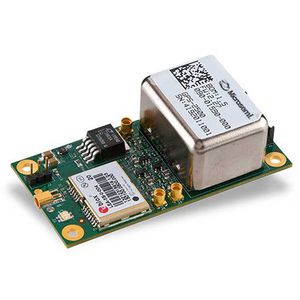
\includegraphics[width=0.5\columnwidth]{figures/gps-2550}
        \caption{Example of a GPSDO based on a OCXO (Microsemi GPS-2550).}
        \label{fig:ex-gpsdo}
    \end{center}
\end{figure}

\subsubsection{Conclusions}

\begin{table}[!ht]
    \centering
    \begin{tabular}{lcccc}
        \toprule[1.5pt]
        \textbf{Oscillator Type} & \textbf{Accuracy} & \textbf{Aging/10 year} & \textbf{Power} & \textbf{Weight} \\
        \midrule
        XO                   & $10^{-5}$ to $10^{-4}$   & 10-20 PPM                                 & 20 $\mu$W  & 20 g \\
        TXCO                 & $10^{-6}$                & 2-5 PPM                                   & 100 $\mu$W & 50 g \\
        MCXO                 & $10^{-8}$ to $10^{-7}$   & 1-3 PPM                                   & 200 $\mu$W & 100 g \\
        OCXO (5 to 10 MHz)   & $10^{-8}$                & $2 \times 10^{-8}$ to $2 \times 10^{-7}$  & \multirow{2}{*}{1-3 W} & \multirow{2}{*}{200-500 g} \\
        OCXO (15 to 100 MHz) & $5 \times 10^{-7}$       & $5 \times 10^{-10}$ to $5 \times 10^{-9}$ &            &  \\
        RbXO                 & $10^{-9}$                & $5 \times 10^{-10}$ to $5 \times 10^{-9}$ & 6-12 W & 1,5-2,5 kg\footnote{\textcolor{red}{Há versões miniaturiazadas.}} \\
        Cs                   & $10^{-12}$ to $10^{-11}$ & $10^{-12}$ to $10^{-11}$                  & 25-40 W & 10-20 kg \\
        GPS                  & $4 \times 10^{-8}$ to $10^{-11}$ & $10^{-13}$ & 4 W & 340 g \\
        \bottomrule[1.5pt]
    \end{tabular}
    \caption{Compasiron between the main types of oscillators \cite{mancini2004}.}
    \label{tab:osc-comp}
\end{table}

\begin{itemize}
    \item Adicionar transmissão de sinais de GNSS às mega-constelações atuais, precisando somente adicionar relógio de alta precisão a cada satélite. Considerando custo e praticidade, essa seria possivelmente a melhor alternativa.
    \item Montar uma rede dedicada, com satélites feitos exclusivamente para emissão de sinais de GNSS. Essa seria solução de maior custo e provavelmente a mais ineficiente em termos de praticidade.
\end{itemize}

\subsection{Radio transmitters}

%Como discutido na \autoref{sec:ionospheric-delay}, uma solução para contornar o problema do atraso ionosférico é a utilização de duas frequências diferentes para a transmissão dos sinais de geolocalização. Com isso, surge a necessidade da utilização de dois transmissores diferentes, ou até mesmo um único transmissor com a capacidade de realizar transmissões em duas frequências distintas.

%Neste caso, não há grandes requisitos técnicos para um transmissor deste tipo. Mas, alguns cuidados devem ser tomados a utilização neste tipo de sistema. Um deles é com o tempo de duração das transmissões, já que em um sistema deste tipo, o rádio deve emitir sinais a todo momento, deste forma o mesmo deve suportar operações ininterruptas. Neste caso, deve-se tomar cuidado com o projeto térmico do mesmo, já em operando desta forma, calor considerável seria gerado o que poderia diminuir a vida útil dos circuitos ou até mesmo danificá-los permanentemente. Ou cuidado a ser tomado, e neste caso especialmente tratando-se da utilização em satélites de pequeno porte, seria em relação ao consumo energético dos transmissores. Considerando transmissões com alta periodicidade ou até mesmo ininterruptas, a eficiência energética do transmissor torna-se extremamente relevante.

%Considerando uma operação nas frequências já utilizadas pelas redes de GNSS atuais, também haveria a necessidade da utilização de transmissores customizados, pois para estas frequências normalmente não se encontra transmissores COTS para satélites no mercado.

%Devido às variações térmicas que um satélite está exposto, também podem ocorrer drifts de frequência no circuito de clock do transmissor, causando variações na frequência dos sinais transmitidos. Desta forma, também deve-se utilizar circuitos com boa precisão. Mas diferentemente dos circuitos de clock da referência de tempo do sistema, altas precisões como a encontrada em relógio de rubídio ou césio, por exemplo, não são necessárias.

%Considerando os aspectos térmicos, energéticos e de operação, uma solução customizada para o rádio transmissor seria a mais indicada. Uma outra possibilidade seria a utilização de um Rádio Definido por Software (SDR), onde neste caso a maior parte das etapas de transmissão poderiam ser implementadas em software.

The solution to overcome the ionospheric delay problem discussed in \autoref{sec:ionospheric-delay} is the use of two different frequencies for geolocation signal transmission. This creates the need for two different transmitters, or even a single transmitter with the ability to transmit on two different frequencies.

There are no major technical requirements for this type of transmitter. However, some precautions must be taken when using it in this type of system. One of them is the duration of transmissions, as the radio must emit signals continuously, so the design must consider the thermal management to avoid reducing the lifespan of the circuits or even damaging them permanently.

Another aspect to consider, especially for use in small satellites, is the energy consumption of the transmitters. Considering transmissions with high periodicity or even continuous, the energy efficiency of the transmitter becomes extremely relevant.

Customized transmitters would be necessary for operation at the frequencies currently used by existing GNSS networks, as COTS transmitters for satellites are not usually available for these frequencies in the market. Due to the thermal variations to which a satellite is exposed, frequency drifts in the transmitter's clock circuit may occur, causing variations in the frequency of the transmitted signals. Therefore, circuits with good precision must be used, but high precision like that found in rubidium or cesium clocks is not necessary.

Considering the thermal, energy, and operational aspects, a custom solution for the transmitter would be the most appropriate. Another possibility would be the use of a Software Defined Radio (SDR), where most of the transmission stages could be implemented in software.

\subsection{Antenna}

%Para as antenas dos transmissores, dependendo da frequência adotada, diferentes geometrias e tipos de antenas podem ser utilizadas. Considerando as frequências utilizadas nos sistemas de GNSS atualmente em funcionamento, antenas do tipo Patch podem ser uma boa opção. Considerando por exemplo satélite seguindo o padrão CubeSat, antenas desse tipo são ideias, pois se adequam ao tamanho físico disponível nesse tipo de satélite, e normalmente não requerem mecânismos de ejeção ou abertuda de componentes, que dificultam o projeto das mesmas e trazem riscos durante a fase de comissionamento do satélite.

%Novamente, considerando o uso das frequências normalmente utilizadas em sistemas de GNSS, há a necessidade do projeto de uma antena customizada, pois normalmente não há disponível no mercado antenas Patch para satélite de pequeno porte e que operem nessa faixa de frequência.

For transmitter antennas, different geometries and types of antennas can be used depending on the adopted frequency. Considering the frequencies used in currently operating GNSS systems, Patch antennas can be a good option. For example, for satellites following the CubeSat standard, these types of antennas are ideal because they fit the physical size available in this type of satellite and usually do not require mechanisms for ejecting or opening components, which can complicate their design and pose risks during the satellite commissioning phase.

Again, considering the use of frequencies typically used in GNSS systems, there is a need for a custom-designed antenna because Patch antennas for small satellites operating in this frequency range are not usually available on the market.

\subsection{Attitude and orbit control}

%Considerando as características já apresentadas, para um sistema como esse, não se tem a necessidade de um sistema de controle de atitude altamente preciso, como por exemplo os tipos empregados em satélites para imageamento. Já que os requisitos de operação em relação a atitude se limitam basicamente a manter as antenas voltadas para o Terra durante toda a órbita, um sistema com baixa precisão já seria suficiente. Possivelmente um sistema de controle ativo com magnetorquers em um satélite pequeno seria suficiente, onde nesse caso pode-se atingir uma precisão de até \textcolor{red}{XX} graus. Para satélites maiores, sistemas com rodas de reação podem ser necessários.

%Já em relação ao controle de órbita, devido a natureza de operação na forma de constelação de sistemas desse tipo, um controle da posição do satélite ao longo da sua órbita é necessário. Manter os satélites da constelação em órbitas específicas e principalmente distantes entre si é um fator importante para o correto funcionamento do sistema, visando principalmente a na ocorrência de zonas mortas, onde não há satélites transmitindo sinais em determinados momentos.

%Para isso, alguns tipos de sistemas podem ser utilizados, como por exemplo propulsores baseados na emissão de íons e/ou propulsores a base de propelentes. Novamente, tratando-se de satélites de pequeno porte, aspectos energéticos e físicos devem ser levados em conta para sistemas desse tipo. Por exemplo, sistemas baseados em propelentes podem ser de difícil utilização, devido ao pouco espaço físico disponível para o armazenamento do material propelente.

Considering the characteristics presented, for a system like this, there is no need for a highly precise attitude control system, such as those used in imaging satellites. Since the attitude operation requirements are limited to keeping the antennas pointing towards Earth throughout the orbit, a low-precision system would be sufficient. An active control system with magnetorquers on a small satellite would possibly be sufficient, where in this case, a precision of up to 20 degrees could be achieved \cite{carrara2017}. For larger satellites, reaction wheel systems may be necessary.

Regarding orbit control, due to the nature of operation in the form of a constellation of systems like this, control of the satellite's position along its orbit is necessary. Maintaining the constellation satellites in specific and mainly distant orbits from each other is an important factor for the correct functioning of the system, mainly aiming to avoid dead zones where no satellites transmit signals at certain times.

For this purpose, some types of systems can be used, such as ion thruster-based and/or propellant-based thrusters. Again, for small satellites, energy and physical aspects must be taken into account for these types of systems. For example, propellant-based systems may be difficult to use due to the limited physical space available for storing the propellant material.

\begin{figure}[!ht]
    \begin{center}
        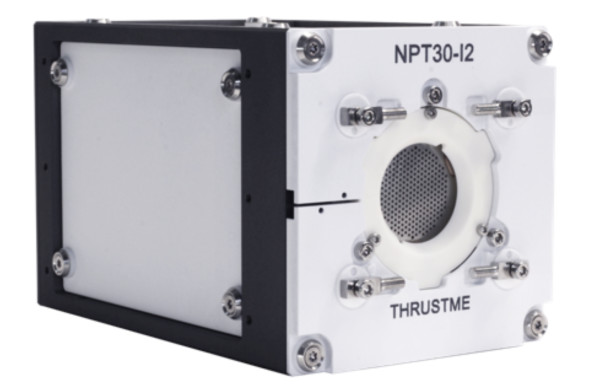
\includegraphics[width=0.5\columnwidth]{figures/npt30-i2}
        \caption{NPT30-I2 ion thruster from ThrustMe.}
        \label{fig:thrustme-npt30-i2}
    \end{center}
\end{figure}

\section{Proposed experiment}

%Como forma de testar o trabalho proposto, propõe-se o desenvolvimento de uma carga útil voltada para pequenos satélites (e neste caso já compatível com o padrão CubeSat). Seguindo o que foi discutido até então, esta carga útil será basicamente um módulo de transmissão de sinais de GNSS, que pode ser integrado a um satélite de pequeno porte. A ideia é que este módulo seja composto por duas placas de circuito impresso que podem ser controlados pelo computador de bordo do satélite, onde o mesmo pode controlar o funcionamento da mesma, e/ou adquirir dados de telemetria a respeito do funcionamento da carga útil.

As a way of testing the proposed work, the development of a payload aimed at small satellites (already compatible with the CubeSat standard in this case) is proposed. Following what has been discussed so far, this payload will basically be a GNSS signal transmission module that can be integrated into a small satellite. The idea is that this module will be composed of two printed circuit boards that can be controlled by the satellite's onboard computer, where it can control its operation and/or acquire telemetry data about the payload's operation.

%Um diagrama de blocos preliminar do módulo proposto pode ser visto na \autoref{fig:payload-block-diagram}. Na \autoref{fig:payload-block-diagram-radios}, há um detalhamento da segunda placa da carga útil, que é composta pelos elementos de radio frequência.

A preliminary block diagram of the proposed module can be seen in \autoref{fig:payload-block-diagram}. In \autoref{fig:payload-block-diagram-radios}, there is a breakdown of the second board of the payload, which is composed of radio frequency elements.

\begin{figure}[!ht]
    \begin{center}
        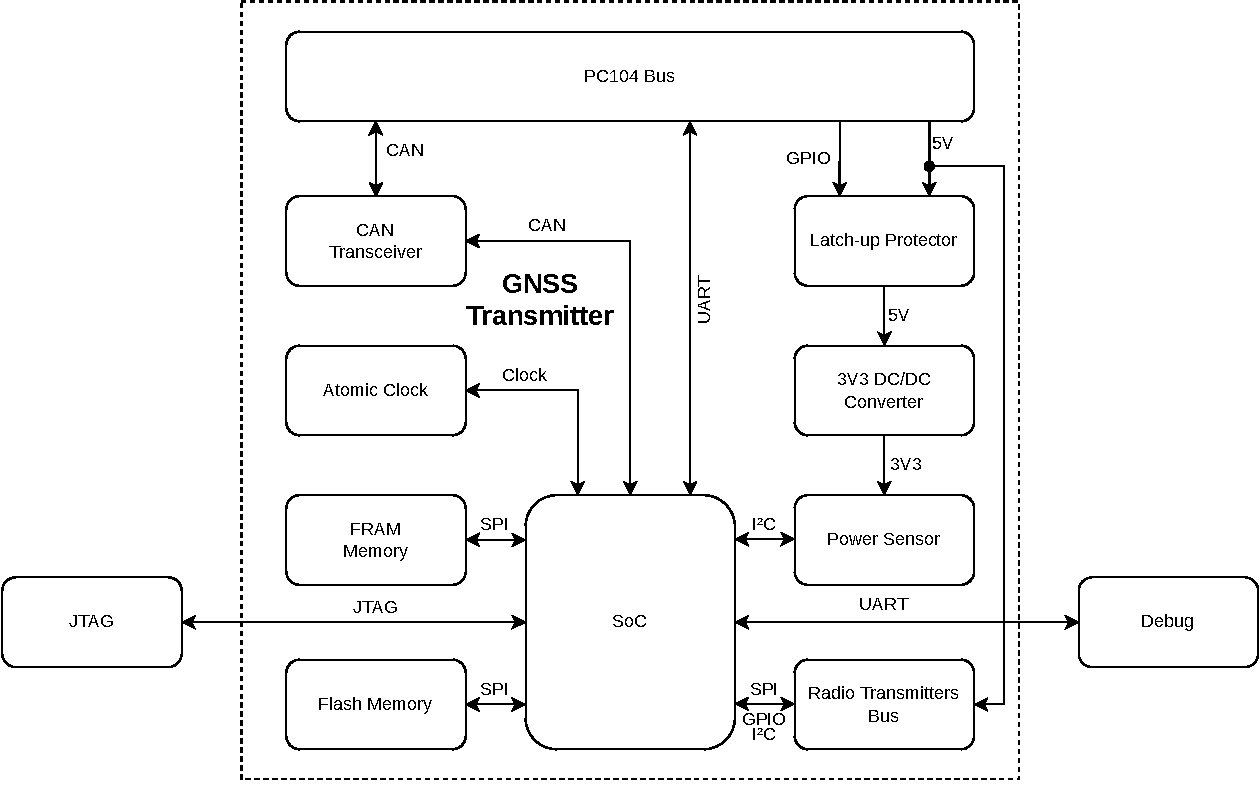
\includegraphics[width=\columnwidth]{figures/block-diagram}
        \caption{Preliminary block diagram of the proposed payload.}
        \label{fig:payload-block-diagram}
    \end{center}
\end{figure}

\begin{figure}[!ht]
    \begin{center}
        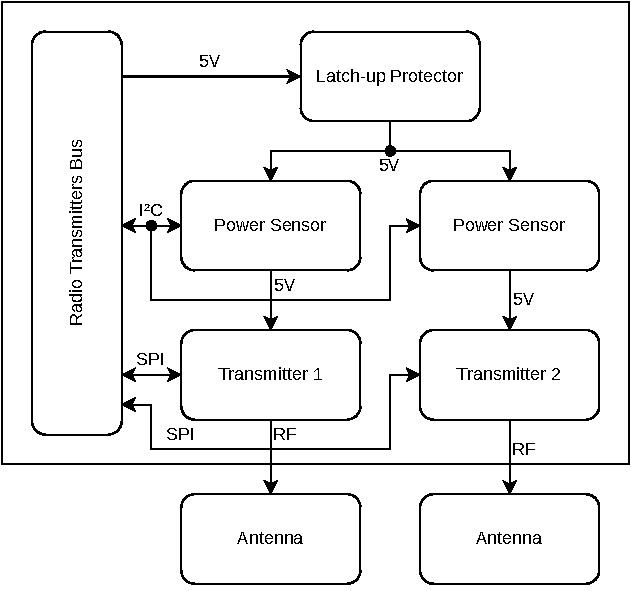
\includegraphics[width=0.6\columnwidth]{figures/radios-block-diagram}
        \caption{Preliminary block diagram of the radio transmitters module.}
        \label{fig:payload-block-diagram-radios}
    \end{center}
\end{figure}

%Como pode ser visto nos diagrama, seguindo algumas características comuns em cargas úteis voltadas para CubeSats, pretende-se utilizar um ou mais barramentos de 5 V para a alimentar todo o conjunto. A comunicação de dados com o restante do satélite (computador de bordo neste caso) poderá ser feita tanto através de um barramento CAN, quanto através de um barramento RS-485. Todas essas entradas e saídas através de um barramento do tipo PC104.

As can be seen in the diagram, following some common characteristics in payloads aimed at CubeSats, one or more 5V buses will be used to power the entire assembly. Data communication with the rest of the satellite (onboard computer in this case) can be done through either a CAN bus or an RS-485 bus. All of these inputs and outputs through a PC104 bus.

%Internamente, a linha de alimentação será composta num primeiro estágio por um proteto contra latch-up, que limitam a corrente de entrada do circuito e protegem contra possíveis surtos de corrente causados por radiação solar e que podem danificar permanentemente o módulo. Desta forma, a adição de uma proteção contra latch-ups pode aumentar o tempo de funcionamento dos elementos do circuito \cite{botma2013}. Após esta etapa, encontra-se um conversor DC/DC que abaixa os 5 V de entrada para 3.3 V, que é a tensão de alimentação principal da maior parte dos elementos da placa. Após a etapa de conversão de tensão, encontra-se um sensor de tensão e corrente, que permite acompanhar o consumo de energia da parte de processamento e controle do módulo. Este sensor é controlado e acessado pelo processador principal do módulo.

Internally, the power line will be composed in a first stage by a latch-up protection, which limits the input current of the circuit and protects against possible current surges caused by solar radiation that can permanently damage the module. Thus, adding latch-up protection can increase the operating time of the circuit elements. After this stage, there is a DC/DC converter that lowers the 5V input to 3.3V, which is the main supply voltage for most of the board's components. After the voltage conversion stage, there is a voltage and current sensor that allows monitoring of the processing and control part's energy consumption. This sensor is controlled and accessed by the module's main processor.

%Para a parte de controle, será utilizado um SoC (System-on-a-chip) composto por um microcontolador e um FPGA. O modelo exato do mesmo ainda está sob análise. Este elemento será responsável por coordenar todo o funcionamento da carga útil, e por realizar a comunicação com o computador de bordo do satélite.

For the control part, a SoC (System-on-a-chip) composed of a microcontroller and an FPGA will be used. The exact model is still under analysis. This element will be responsible for coordinating the entire payload's operation and for communicating with the satellite's onboard computer.

%Na parte de memórias externas, será utilizado prelinimarmente um memória RAM do tipo FRAM, para armazenamento de dados críticos da carga útil (como por exemplo parâmetros de configuração). Também pretende-se utilizar uma memória flash do tipo NAND para armazenamento de dados em massa (neste caso, dados de telemetria).

For external memory, an FRAM type RAM will be preliminarily used to store critical payload data (such as configuration parameters). It is also intended to use a NAND flash memory for mass data storage (in this case, telemetry data).

%Na parte de sensoriamento, como já citado anteriormente, pretende-se utilizar um sensor de tensão e corrente, além de um sensor de temperatura instalado próximo ao circuito de referência de clock.

For sensing, as mentioned earlier, a voltage and current sensor will be used, as well as a temperature sensor installed near the clock reference circuit.

%Já na parte do circuito de referência de clock, será utilizar um relógio atômico de rubídio, como já discutido anteriormente neste capítulo. O sinal de referência gerado alimentará um circuito digital implementado no FPGA do SoC utilizado, e servirá como referência para o relógio interno do sistema.

In the clock reference circuit part, a rubidium atomic clock will be used, as discussed earlier in this chapter. The reference signal generated will feed a digital circuit implemented in the SoC's FPGA used and serve as a reference for the system's internal clock.

%Além disso, a placa também terá transceptores para os barramentos de comunicação: CAN e RS-485.

In addition, the board will also have transceivers for communication buses: CAN and RS-485.

%Já na parte de transmissão dos sinais de rádio frequência, devido a limitações de espaço físico, pretende-se utilizar uma segundo placa acoplada a principal através de um barramento. Esta placa conterá os dois transmissores de rádio do sistema, juntamente com um protetor de latch-up exclusivo para o conjunto, e um sensor de corrente e tensão para cada transmissor, que servirá para acompanhar o funcionamento dos mesmos. Na saída dos transmissores, haverá conectores coaxiais que serviram para conector uma antena ao conjunto. Como estes transmissores irão irradiar sinais com uma potência relativamente elevada, um cuidado especial com a dissipação térmica do mesmo deverá ser levado em conta. Dissipadores de metal deverão ser instalados ao conjunto para dissipar o calor gerado por condução términa. Um sensor de temperatura instalado nesse dissipador poderá auxiliar no monitoramento da temperatura, podendo até servir como alarme e um possível desligamento em caso de superaquecimento do sistema. Problemas de temperatura serão críticos nesse módulo devido principalmente a natureza de um sistema de GNSS: os sinais são transmitidos o tempo todo.

For radio frequency signal transmission, due to physical space limitations, a second board attached to the main one via a bus will be used. This board will contain the system's two radio transmitters, along with an exclusive latch-up protector for the assembly and a voltage and current sensor for each transmitter, which will serve to monitor their operation. At the transmitter's output, there will be coaxial connectors that will connect an antenna to the assembly. As these transmitters will radiate signals with a relatively high power, special care must be taken with their thermal dissipation. Metal heat sinks should be installed on the assembly to dissipate the heat generated by thermal conduction. A temperature sensor installed in this heat sink will allow monitoring the temperature of the system.

%Para auxiliar na proteção contra radiação espacial e na dissipação térmica de todo o módulo, todas as placas serão instaladas dentro de um case de metal (preliminarmente alumínio).

To assist in protection against space radiation and thermal dissipation of the entire module, all boards will be installed within a metal case (preliminarily aluminum).

%Por fim, como já citado, o módulo proposto e descrito ainda encontra-se em fase preliminar de definição, e pode sofrer alterações de acordo com o andamento do trabalho e com resultados preliminares obtidos.

Finally, as already mentioned, the proposed and described module is still in a preliminary stage of definition, and may undergo changes according to the progress of the work and preliminary results obtained.